\FloatBarrier
\section{Wave input, unstructured meshes and robustness}
\label{sec:ext}

This section tests what was added after the comparisons with NHWAVE: the
boundary wavemaker with active absorption, the return current, irregular
waves and measured records (Section~\ref{sec:zones}), with the composite
beach of NTHMP benchmark 5, the model on triangulated meshes, and the
checks that keep the code reproducible: parallel runs, restarts and a
regression suite.

\subsection{Boundary wavemaker and active absorption}
\label{sec:wm}

The tests (script \code{wavemaker.py}) use a flat flume ($h = 0.4$ m,
10 layers, $\Delta x = 2$ cm, $\Delta t = 10$ ms) with regular waves of
$H = 2$ cm and $T = 1.5$ s ($kh = 0.96$) unless stated otherwise. Incident
and reflected amplitudes come from a least-squares fit of
$A_j = a_I e^{ikx_j} + a_R e^{-ikx_j}$ to the first harmonic at 30--70
gauges \citep{zelt1992}, with $k$ adjusted to the model's own wave number
(within 0.1\% of linear theory in the runs of progressive waves).

\paragraph{Progressive waves.} With the wavemaker at $x = 0$ and a 6 m
sponge at the far end, the wave height is within 0.7\% of the target over
13.5 m (mean $0.995H$), and the reflection coefficient of the flume is
0.4\%. A 6 m relaxation zone (2.3 wavelengths) gives $0.998H$ and 0.16\%
(Fig.~\ref{fig:wm-reg}a), with a domain 6 m longer.

\paragraph{Closed flume.} With a wall 10 m from the wavemaker, the waves
reflected by the wall return to the wavemaker. With active absorption the
incident amplitude settles at $1.03\,a$ within 5 periods and stays there for
the 60 periods of the run, with a standing wave of $a_R/a_I = 0.99$ in
front of the wall. Without absorption the wavemaker reflects the returning
waves, which beat with the generated ones: the incident amplitude swings
between $0.1\,a$ and $1.1\,a$ with a period of about 40 s
(Fig.~\ref{fig:wm-reg}b). The 3\% excess with absorption is the
re-reflection of the shallow-water absorber at this $kh$ (below).

\paragraph{Absorbing boundary.} The same condition with zero wave height
lets waves out of the domain. Regular waves made by a 6 m relaxation zone
and absorbed 8 m further on give the reflection coefficients of
Table~\ref{tab:wm-abs} and Fig.~\ref{fig:wm-abs}. With the shallow-water
celerity the reflection follows the estimate
$(1 - c/\sqrt{gh})/(1 + c/\sqrt{gh})$, the mismatch between the imposed
depth-averaged velocity $\sqrt{g/h}\,\eta$ and that of the wave,
$c\,\eta/h$: 1.9\% at $kh = 0.53$, 5.9\% at 0.96 and 12.6\% at 1.72. With
the phase speed of the waves (\code{absorptionCelerity wave}) the
depth-averaged velocity matches, and the reflection falls to 0.3\% and
1.7\% for $kh \le 1$; for shorter waves a correction that is uniform over
the depth cannot match the profile of the wave (9.3\% at $kh = 1.72$). A
sponge layer of 2--5 wavelengths reflects less than 0.5\%, at the cost of
the domain.

\begin{table}[!htbp]
\centering
\caption{Reflection coefficient of the absorbing boundary and of an 8 m
sponge layer, regular waves of $H = 2$ cm in $h = 0.4$ m.}
\label{tab:wm-abs}
\small
\begin{tabular}{ccccc}
\toprule
$T$ & $kh$ & \code{absorptionCelerity shallow} & \code{absorptionCelerity wave} & 8 m sponge \\
\midrule
2.5 s & 0.53 & 1.9\% & 0.3\% & 0.2\% \\
1.5 s & 0.96 & 5.9\% & 1.7\% & 0.4\% \\
1.0 s & 1.72 & 12.6\% & 9.3\% & $<0.1$\% \\
\bottomrule
\end{tabular}
\end{table}

\paragraph{Return current.} In a closed flume of constant depth (a 6 m
wave-making zone, a wall 10 m further on) the mean water level of the flume
stays within 0.1 mm of still water with or without the return current
(Fig.~\ref{fig:wm-reg}c), and within 0.2 mm with the boundary wavemaker and
absorption: the zone relaxes the surface to the target, so the missing
return current only steps the mean level inside the zone. Over the
submerged bar it matters (Section~\ref{sec:bar-bc}).

\begin{figure}[!htbp]
\centering
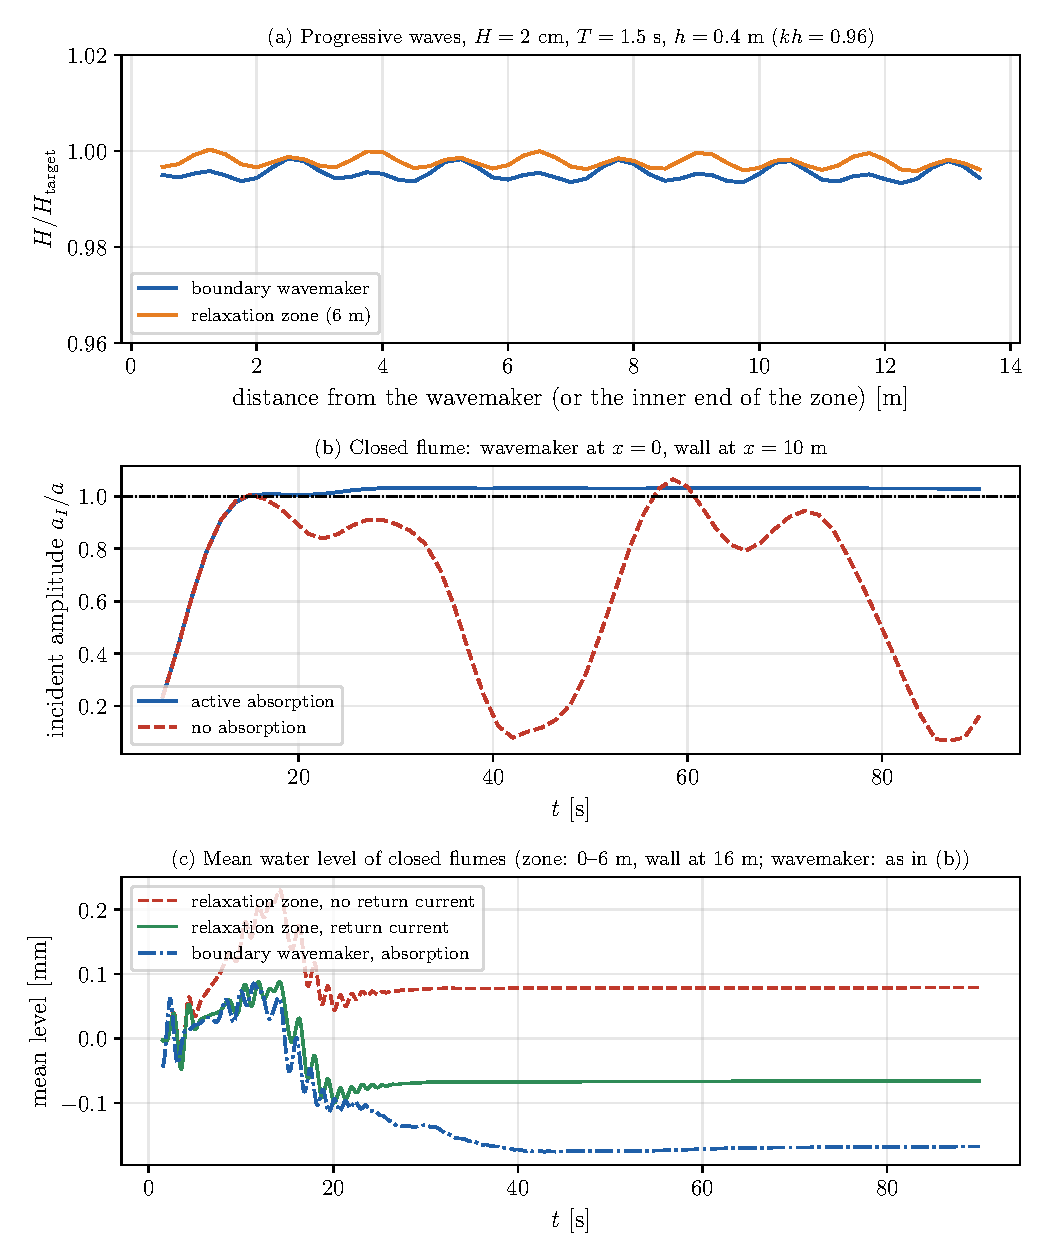
\includegraphics[width=0.85\textwidth]{wavemaker_regular.pdf}
\caption{Wave input in a flat flume ($h = 0.4$ m, $H = 2$ cm, $T = 1.5$ s):
(a) wave height from the boundary wavemaker and from a relaxation zone;
(b) incident amplitude in a closed 10 m flume with and without active
absorption; (c) the mean water level of closed flumes with a relaxation
zone (with and without the return current) and with the wavemaker of (b).}
\label{fig:wm-reg}
\end{figure}

\begin{figure}[!htbp]
\centering
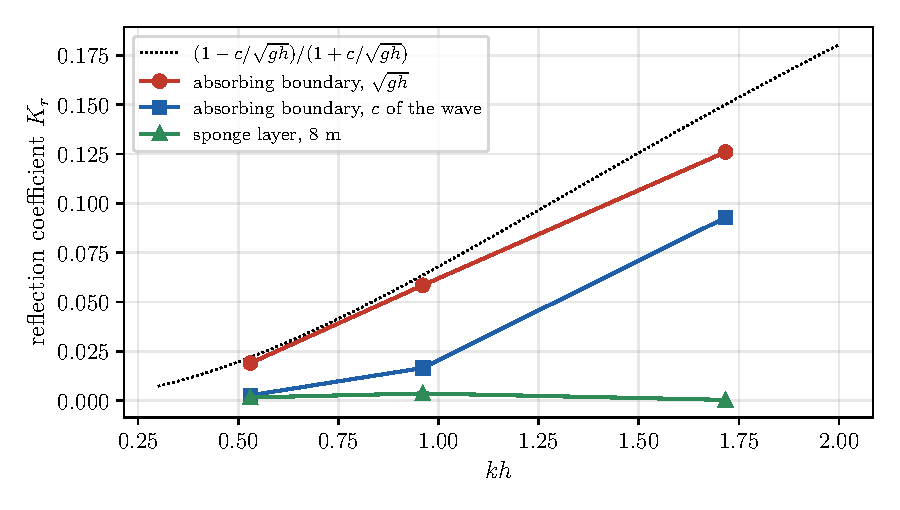
\includegraphics[width=0.65\textwidth]{wavemaker_absorber.pdf}
\caption{Reflection coefficient of the absorbing boundary (\code{nhWaveVelocity}
with zero wave height) with the shallow-water celerity and with the phase
speed of the waves, and of an 8 m sponge layer; the dotted line is the
depth-averaged estimate for the shallow-water absorber.}
\label{fig:wm-abs}
\end{figure}

\subsection{Irregular waves}
\label{sec:irr}

JONSWAP waves ($H_s = 3$ cm, $T_p = 1.5$ s, $\gamma = 3.3$, 100 components
between $0.5f_p$ and $3f_p$, random phases) were made in the same flume by a
6 m relaxation zone and by the boundary wavemaker, and the spectra were
computed at six gauges over 200 s (Welch, 40 s segments;
Fig.~\ref{fig:wm-irr}). Both keep the shape of the target spectrum and its
peak period (1.47 s, the frequency resolution of the spectra), and $H_{m0}$
stays within $-4\%$ and $+2\%$ of the target over 12 m (8 peak
wavelengths). In all runs $H_{m0}$ falls by 3--5\% between 2 and 12 m from
the generator. The loss is in the peak band (0.6--0.75 Hz: 18\% of its
energy over 10 m), it is the same with filtered central convection as with
the TVD scheme, and regular waves of the peak period and 2 cm height do
not show it; its cause is not yet identified.

\begin{figure}[!htbp]
\centering
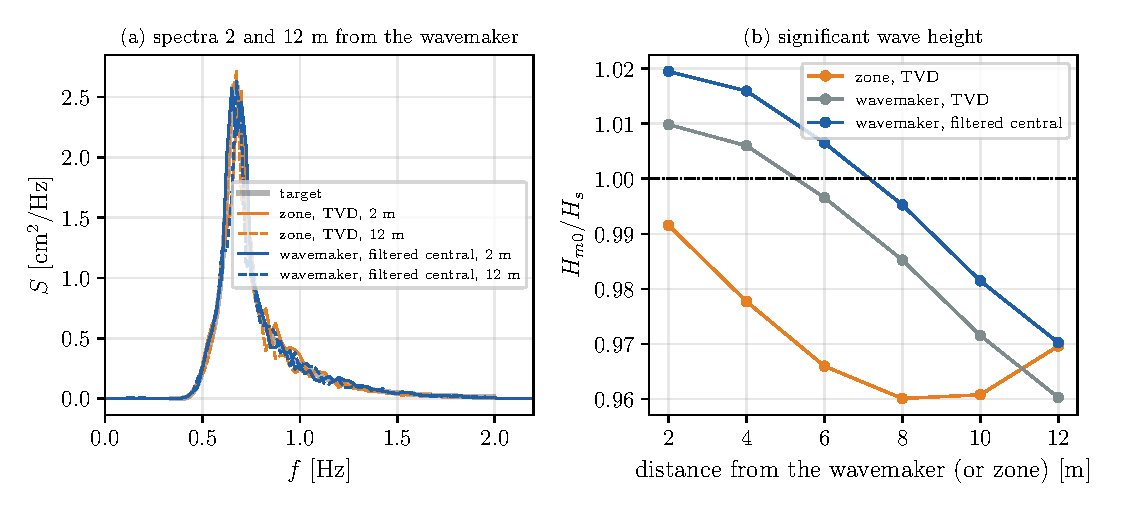
\includegraphics[width=\textwidth]{wavemaker_irregular.pdf}
\caption{JONSWAP waves ($H_s = 3$ cm, $T_p = 1.5$ s, $\gamma = 3.3$, 100
components) from a relaxation zone and from the boundary wavemaker:
(a) spectra 2 and 12 m from the generator against the target; (b) $H_{m0}$
along the flume.}
\label{fig:wm-irr}
\end{figure}

\subsection{The submerged bar: return current and long waves}
\label{sec:bar-bc}

In case C of the submerged bar (Section~\ref{sec:bar10}) the phase of the
waves over the bar drifted during the run, and with it the rms error
(Table~\ref{tab:barwindow}). The case was rerun on the same mesh with the
8 m wave-making zone and the return current, and with the boundary
wavemaker at $x = 0$ (active absorption and return current) in place of
the zone (Table~\ref{tab:bar-bc}, Fig.~\ref{fig:bar-bc}).

\begin{table}[!htbp]
\centering
\caption{Submerged bar, case C, 10 layers: rms error over the 10 gauges for
windows ending at 45--65 s, the time lag of the first harmonic at
$x = 35.7$ m behind $x = 22$ m from the window ending at 45 s to that
ending at 65 s (NHWAVE: 60 s), and the spread of the mean water level over
the gauges.}
\label{tab:bar-bc}
\small
\setlength{\tabcolsep}{3.5pt}
\begin{tabular}{lccccccc}
\toprule
 & \multicolumn{5}{c}{rms error (cm), window ending at} & lag (s) & mean level \\
\cmidrule(lr){2-6}
 & 45 s & 50 s & 55 s & 60 s & 65 s & 45 $\to$ 65 s & spread (mm) \\
\midrule
zone, no return current (Sec.~\ref{sec:bar10}) & 0.49 & 0.65 & 0.94 & 1.18 & 1.39 & $0.98 \to 1.19$ & 1.9--3.6 \\
zone, return current & 1.03 & 1.01 & 1.00 & 1.00 & 1.03 & $0.83 \to 0.84$ & 0.7--0.8 \\
boundary wavemaker & 0.90 & 0.99 & 1.00 & 0.98 & 0.98 & $0.86 \to 0.85$ & 0.7--2.5 \\
NHWAVE & 1.08 & 1.02 & 0.97 & 0.89 & 0.77 & $0.80 \to 0.84$ & 0.9--2.1 \\
REEF3D::NHFLOW & 0.93 & 0.92 & 0.92 & 0.98 & 1.10 & $0.85 \to 0.78$ & 0.9--1.6 \\
lab & & & & & & 0.96 & \\
\bottomrule
\end{tabular}
\end{table}

The drift came from the missing return current. A wave-making zone without
it imposes no mean flow, while the waves carry the Stokes transport into the
closed flume, which must return as a mean current; the mismatch drives mean
currents and long waves, which shift the waves over the 0.1 m deep crest.
With the return current, in the zone or at the wavemaker, the lag no longer
drifts (0.01 s in 20 s instead of 0.21 s), the mean water level varies by
less than 1 mm along the flume once the wave train has passed, and the
error is about 1.0 cm in every window. \NHFOAM\ then has the waves 0.12 s
early at $x = 35.7$ m, like NHWAVE and REEF3D::NHFLOW (0.1--0.18 s); the
smaller errors of the run without the return current in short windows came
from the drift passing through the measured phase. The test of a closed
flume of constant depth (Fig.~\ref{fig:wm-reg}c) is not sensitive to the
return current, because there the mismatch only steps the mean level inside
the zone, by a fraction of a millimetre.

\begin{figure}[!htbp]
\centering
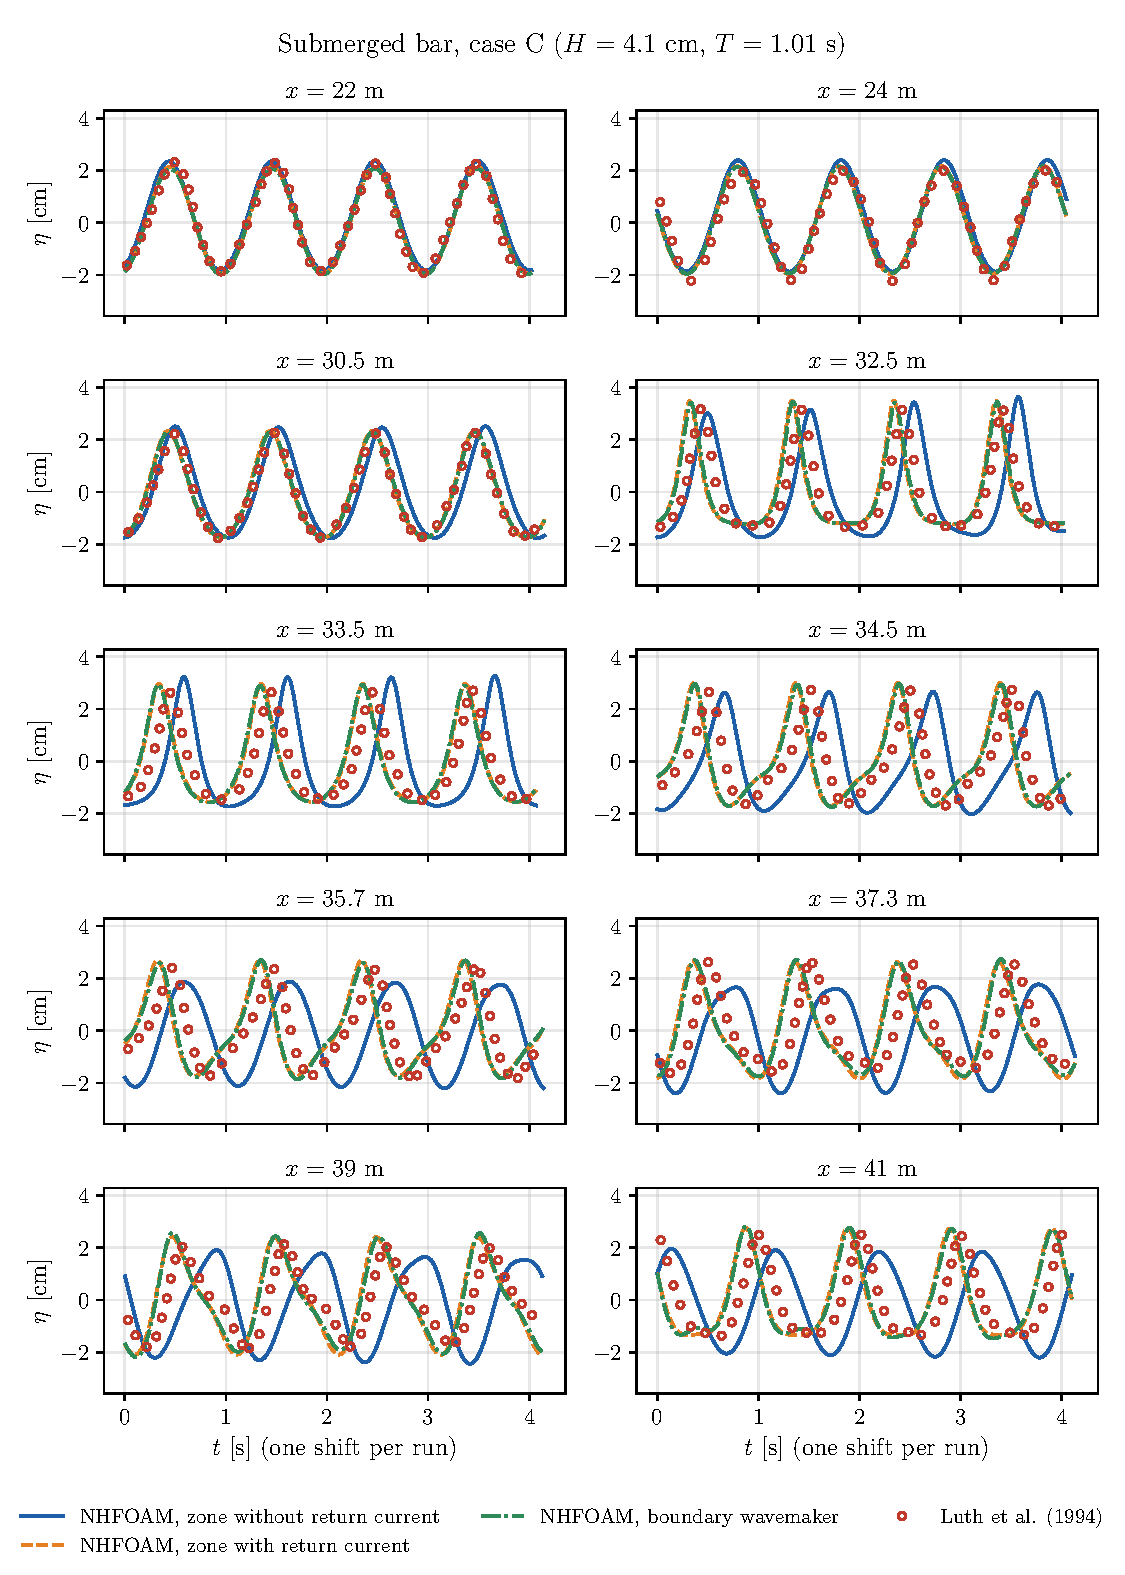
\includegraphics[width=0.9\textwidth]{bar_bc_C.pdf}
\caption{Submerged bar, case C, 10 layers, window ending at 65 s: the
wave-making zone without and with the return current, and the boundary
wavemaker, against \citet{luth1994}.}
\label{fig:bar-bc}
\end{figure}

\subsection{Measured records}
\label{sec:ts}

The time-series input \eqref{eq:timeseries} was first checked on a wave
whose answer is known (script \code{timeseries\_input.py}): a solitary wave
of $H/h = 0.1$, 0.3 and 0.6 is made at $x = 0$ of a flat tank ($h = 0.218$ m,
$\Delta x = 2$ cm, 5 layers, $\Delta t = 5$ ms, a 3 m sponge at the far end)
from its own record, sampled every 0.02 s like a gauge, and compared 12 m
downstream with the exact wave of Babenko's equation. The elevation record
runs with the active absorption, the paddle record (the time integral of
$c\,\eta/(h+\eta)$) without it; for reference the same wave also starts as
the exact initial condition (Table~\ref{tab:ts}, Fig.~\ref{fig:ts}).

\begin{table}[!htbp]
\centering
\caption{Solitary wave made from its record at $x = 0$, 12 m downstream:
crest height, arrival of the crest and rms difference over the pulse
against the exact wave.}
\label{tab:ts}
\small
\begin{tabular}{llccc}
\toprule
$H/h$ & input & crest$/H$ & arrival & rms$/H$ \\
\midrule
0.1 & exact initial condition & 1.000 & $-9$ ms & 0.4\% \\
0.1 & elevation, $c = \sqrt{g(h+\eta)}$ & 0.993 & $-2$ ms & 0.3\% \\
0.1 & elevation, $c$ of the wave & 0.997 & $-7$ ms & 0.3\% \\
0.1 & paddle & 1.000 & $-9$ ms & 0.4\% \\
\midrule
0.3 & exact initial condition & 0.997 & $-6$ ms & 0.6\% \\
0.3 & elevation, $c = \sqrt{g(h+\eta)}$ & 0.979 & $+17$ ms & 1.8\% \\
0.3 & elevation, $c$ of the wave & 0.995 & $-3$ ms & 0.3\% \\
0.3 & paddle & 0.996 & $-3$ ms & 0.2\% \\
\midrule
0.6 & exact initial condition & 0.980 & $+3$ ms & 0.5\% \\
0.6 & elevation, $c = \sqrt{g(h+\eta)}$ & 0.991 & 0 ms & 0.5\% \\
0.6 & elevation, $c$ of the wave & 1.037 & $-58$ ms & 9.5\% \\
0.6 & paddle & 0.937 & $+56$ ms & 8.1\% \\
\bottomrule
\end{tabular}
\end{table}

Up to $H/h = 0.3$ the input with the celerity of the wave, and the paddle
record, are as good as the exact initial condition: crests within 0.5\% of
$H$, arrival within 10 ms after 12 m, trailing waves below 0.1\%
($H/h = 0.1$) and 0.7\% of $H$ ($H/h = 0.3$). The local celerity
$\sqrt{g(h+\eta)}$ of the NTHMP benchmarks carries too little water on the
flanks of the pulse, so the wave of $H/h = 0.3$ comes out 2\% low and 17 ms
late. At $H/h = 0.6$ (with $\Delta t = 4$ ms) a velocity that is uniform
over the depth no longer fills the boundary column under the steep crest:
the paddle record, without absorption, makes the wave 6\% low and 56 ms
late, and with an elevation record the active absorption makes up the
difference, too much with the celerity of the wave (4\% high, 58 ms early)
and about right with the local celerity (1\% low, on time). The local
celerity is therefore the safer choice for steep pulses, and
$\sqrt{g(h+H)}$ the better one for $H/h \le 0.3$.

\begin{figure}[!htbp]
\centering
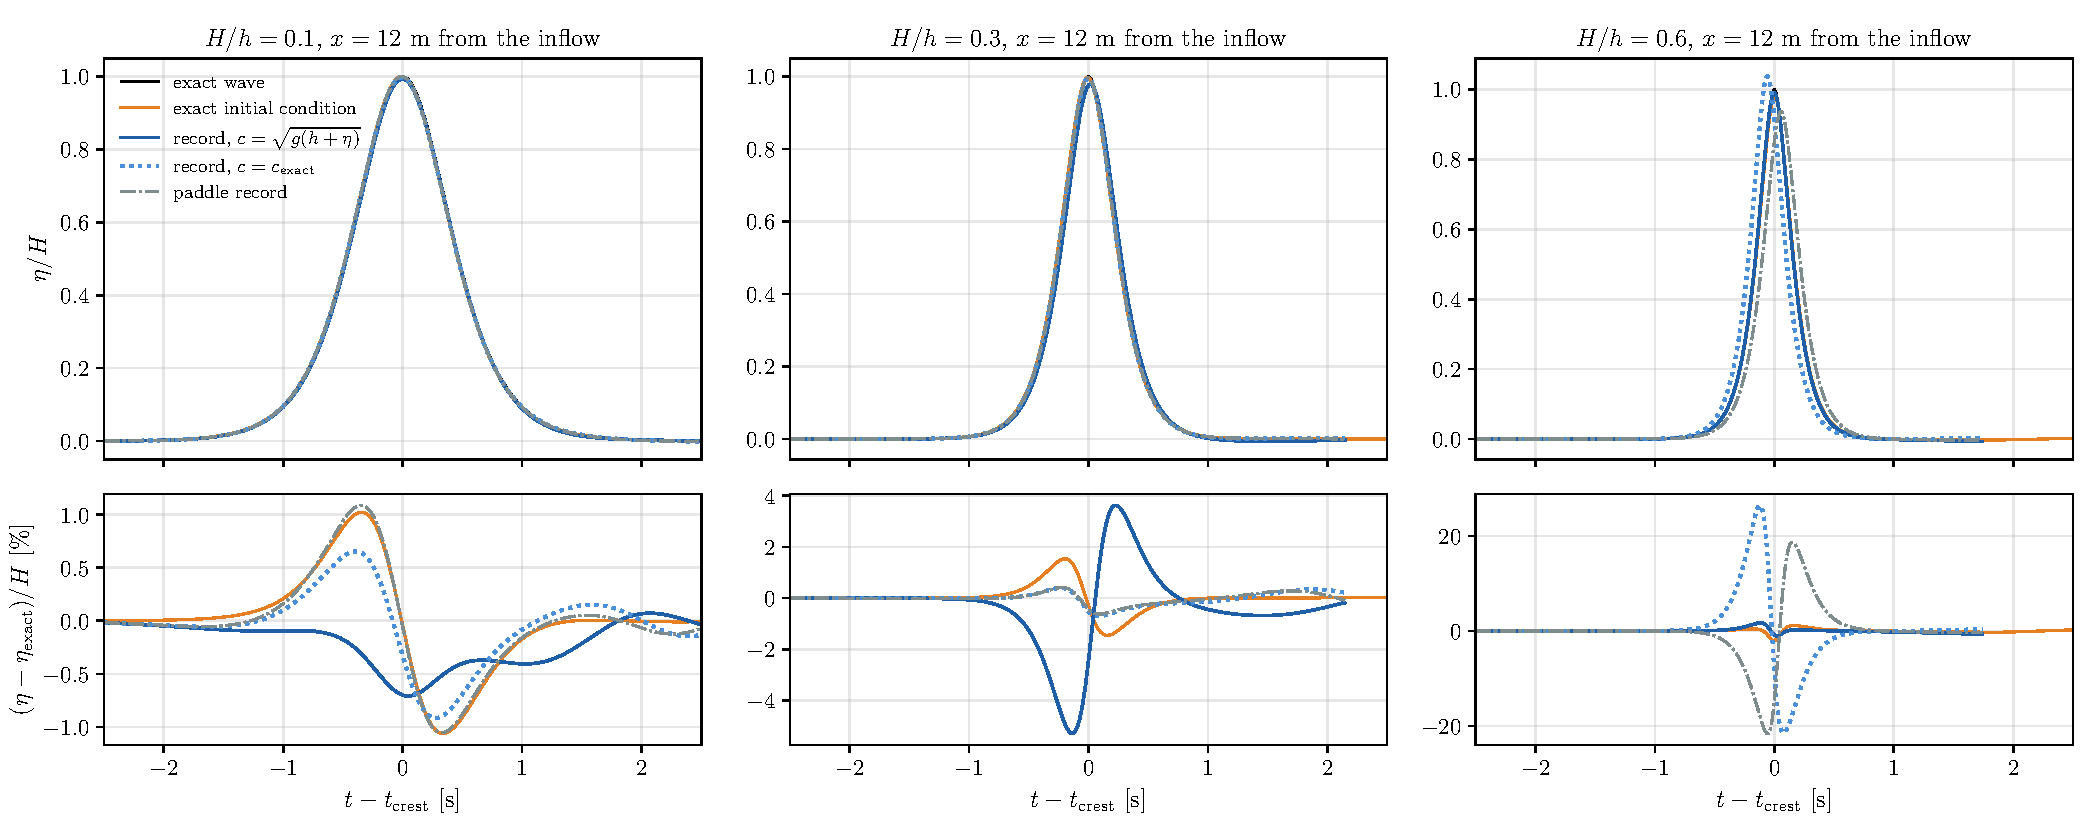
\includegraphics[width=\textwidth]{timeseries_input.pdf}
\caption{Solitary waves made from their records at $x = 0$, 12 m
downstream, against the exact wave: elevation (top) and difference from the
exact wave (bottom).}
\label{fig:ts}
\end{figure}

\subsection{Solitary waves on a composite beach with a vertical wall}
\label{sec:cb}

The Coastal and Hydraulics Laboratory of the US Army Corps of Engineers
built a model of Revere Beach in a flume: 0.218 m of water from the
wavemaker to 15.04 m, then slopes of 1:53, 1:150 and 1:13 up to a vertical
wall at 23.23 m that stands in 4.7 cm of water (benchmark problem 3 of the
1995 long-wave run-up workshop, \citealp{yeh1996}; NTHMP benchmark 5;
\citealp{kanoglu1998} give its linear solution). It is one of the tests of
NHWAVE's tsunami benchmark report \citep{tehranirad2012}. Solitary waves of
target $H/d = 0.05$, 0.30 and 0.70 (cases A, B and C; 0.038, 0.26 and 0.68
at the incident gauge 4) shoal over the slopes, reflect from the wall (B and
C break first) and run back past gauges 4--10, and the highest run-up on
the wall was measured. The benchmark gives the paddle trajectories and
recommends driving the models with the record of gauge 4, which is what the
time-series input is for (script \code{composite\_beach.py}).

Both models use 3 layers, log-law friction with $k_s = 0.1$ mm (NHWAVE's
\code{Zob} in its examples of the inundation benchmarks) and a 5 mm film;
\NHFOAM\ runs its hybrid breaking model. \NHFOAM\ makes the wave in three
ways on a 1 cm grid, the grid of NHWAVE's report: from the record of gauge 4
(the domain starts at the gauge, and the direct pulse, to 275 s, drives
\code{nhWaveVelocity} with the benchmark's velocity relation and the
active absorption), from the paddle record (the whole flume, from the middle
of the paddle stroke, without absorption), and as the exact solitary wave of
the height measured at gauge 4, its crest timed to the measured one there.
The last is also NHWAVE's input. On the 1 cm grid NHWAVE grows short-wave
noise in this flume (wiggles of $\pm1.5$ mm on the 8 mm crest of case A,
crests 3--8\% high, with or without its $k$--$\varepsilon$ model, in a flat
tank as well), so the two models are compared on a 2 cm grid, where NHWAVE
carries the solitary wave cleanly. NHWAVE's $k$--$\varepsilon$ model, on in
its inundation examples, damps the steep waves of cases B and C already on
the flat bed (in a flat tank a wave of $H/d = 0.26$ keeps $0.87H$ after
3.5 m with it and $1.02H$ without it), so NHWAVE runs without it and, for
reference, with it. Table~\ref{tab:cb} and Fig.~\ref{fig:cb} compare the
runs with the measurements; no run is shifted in time.

\begin{table}[!htbp]
\centering
\caption{Composite beach: crests against the measured ones (model/lab $-$ 1,
\%): the incident crest at gauges 4, 5, 7 and 8 (at gauge 4 of the record
run the boundary column against the record), the highest crest at gauges 9
and 10, where the incident and reflected waves overlap, and the reflected
crest at gauge 5; the rms difference over gauges 5--10 from the arrival of
the wave; the highest water level $R$ at the wall. Gauge 10 saturated in
case B.}
\label{tab:cb}
\small
\setlength{\tabcolsep}{3pt}
\begin{tabular}{llrrrrrrrcc}
\toprule
case & run & g4 & g5 & g7 & g8 & g9 & g10 & g5 refl. & rms (cm) & $R$ (cm) \\
\midrule
A & lab & & & & & &  & & & 2.74 \\
A & \NHFOAM, gauge 4 record & 0 & $-$5 & $-$5 & +3 & $-$4 & $-$10 & +10 & 0.08 & 2.30 \\
A & \NHFOAM, paddle record & +27 & +16 & +15 & +25 & +25 & +19 & +40 & 0.19 & 2.76 \\
A & \NHFOAM, solitary, 2 cm & 0 & $-$9 & $-$9 & $-$2 & $-$1 & $-$2 & +8 & 0.11 & 2.13 \\
A & NHWAVE, solitary, 2 cm & +1 & $-$8 & $-$9 & $-$1 & +1 & $-$1 & +14 & 0.11 & 2.16 \\
A & NHWAVE $k$--$\varepsilon$, 2 cm & +1 & $-$8 & $-$9 & $-$1 & +3 & $-$1 & +13 & 0.11 & 2.19 \\
\midrule
B & lab & & & & & & (clipped) & & & 45.7 \\
B & \NHFOAM, gauge 4 record & $-$1 & +10 & $-$7 & $-$1 & +7 &  & +16 & 0.63 & 17.4 \\
B & \NHFOAM, paddle record & +15 & +22 & +7 & +15 & +26 &  & +27 & 1.12 & 18.6 \\
B & \NHFOAM, solitary, 2 cm & $-$1 & +5 & $-$9 & $-$3 & +5 &  & +19 & 0.75 & 18.8 \\
B & NHWAVE, solitary, 2 cm & +5 & +11 & $-$8 & $-$5 & +5 &  & +25 & 0.90 & 19.6 \\
B & NHWAVE $k$--$\varepsilon$, 2 cm & $-$21 & $-$15 & $-$26 & $-$23 & $-$2 &  & $-$7 & 0.27 & 17.5 \\
\midrule
C & lab & & & & & &  & & & 27.4 \\
C & \NHFOAM, gauge 4 record & $-$14 & +12 & $-$18 & +46 & +30 & $-$12 & +27 & 1.34 & 23.8 \\
C & \NHFOAM, paddle record & +7 & +15 & $-$18 & +46 & +28 & $-$12 & +29 & 1.90 & 23.5 \\
C & \NHFOAM, solitary, 2 cm & $-$7 & 0 & $-$17 & +39 & +29 & $-$16 & +20 & 1.08 & 23.6 \\
C & NHWAVE, solitary, 2 cm & $-$20 & +1 & $-$14 & +75 & +34 & $-$11 & +13 & 1.17 & 28.4 \\
C & NHWAVE $k$--$\varepsilon$, 2 cm & $-$21 & $-$15 & $-$15 & +71 & +21 & $-$17 & $-$5 & 0.92 & 24.7 \\
\bottomrule
\end{tabular}
\end{table}

\begin{figure}[!htbp]
\centering
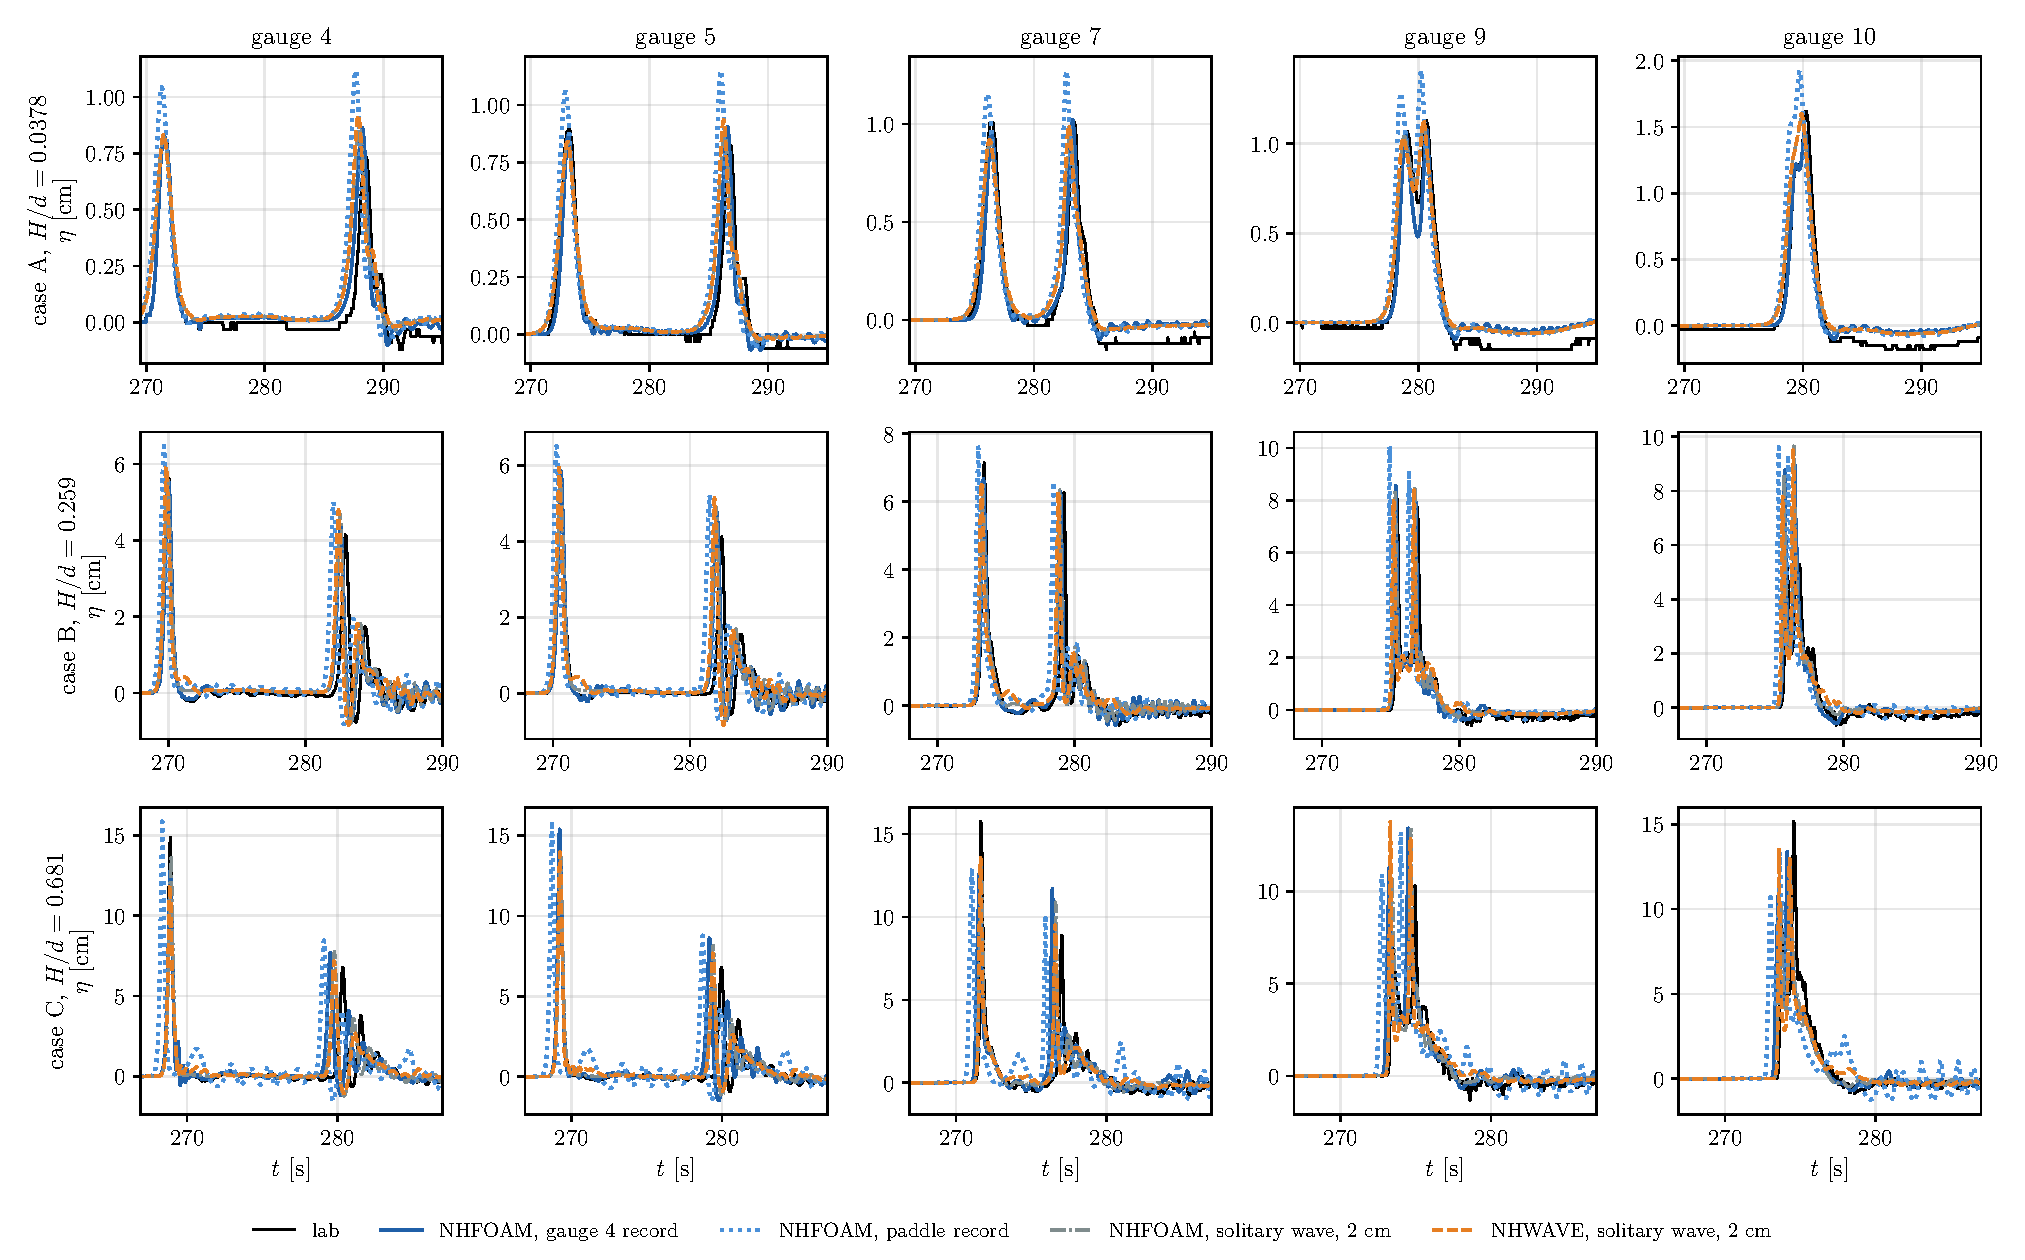
\includegraphics[width=\textwidth]{composite_beach_gauges.pdf}
\caption{Solitary waves on the composite beach, cases A--C (rows), at
gauges 4, 5, 7, 9 and 10: \NHFOAM\ driven by the record of gauge 4 and by
the paddle record (1 cm grid), \NHFOAM\ and NHWAVE (without its
$k$--$\varepsilon$ model) from the exact solitary wave (2 cm grid), against
the measurements.}
\label{fig:cb}
\end{figure}

\paragraph{The record of gauge 4} carries the measured pulse, which is not a
solitary wave: in case A it is 20\% narrower at half height than the
solitary wave of its height (1.25 s against 1.55 s). With it the incident
crests at gauges 5--8 are within 5\% of the measured ones in case A and
within 10\% in case B, they arrive within 0.13 s, and the rms difference is
the smallest of the three inputs (0.08 and 0.63 cm). The benchmark's
velocity and the celerity $\sqrt{g(d+H)}$ give the same crests within 2\% in
these cases. Case C ($H/d = 0.68$) is at the limit of the input: the
boundary column falls 14\% short of the recorded crest (22\% with
$\sqrt{g(d+H)}$), as in the flat tank at $H/h = 0.6$, and the absorption
makes up the volume, so the crest at gauge 5 is 12\% above the measured one.

\paragraph{The paddle record} makes waves 27\%, 15\% and 7\% higher than
measured at gauge 4 (cases A, B, C), which arrive 0.2--0.6 s early. In the
flat tank the paddle input reproduces the wave of a piston that follows its
record to 0.4\% up to $H/h = 0.3$, so the laboratory paddle displaced less
water than its record implies (leakage past the paddle, or the calibration
of its feedback signal; the measured heights also fell short of the target
ones). This is why the benchmark recommends the record of gauge 4.

\paragraph{Breaking.} In case C the measured wave peaks at gauge 7 (19.4 m)
and plunges before gauge 8, while the waves of both models are 14--18\%
lower at gauge 7 (\NHFOAM\ breaks at 16.8--18.4 m) and 39--75\% higher at
gauge 8: the broken waves keep too much height, as on the spilling-breaker
beaches (Section~\ref{sec:brk}).

\paragraph{\NHFOAM\ and NHWAVE} with the same input on the same grid agree
within 2\% at every gauge in case A, where the reflected crest at gauge 5 is
14\% high in NHWAVE and 8\% in \NHFOAM, and the run-up on the wall differs
by 0.03 cm. In case B NHWAVE's crests are within 6\% of \NHFOAM's. In case
C the near-limit wave loses height on the flat bed before gauge 4 in both
models, 20\% in NHWAVE and 7\% in \NHFOAM\ (which does not break there);
after that the two follow the same pattern, and NHWAVE's run-up on the wall
is the closer one (28.4 cm against 23.6 cm, measured 27.4 cm). With its
$k$--$\varepsilon$ model NHWAVE's incident crests are already 21\% low at
gauge 4 in cases B and C; its small rms in case B comes from its slower
wave, which meets the measured arrival times, not from the crests.

\paragraph{The wall and the measurements.} The run-up on the wall is 16\%
low in case A (2.30 against 2.74 cm) and 13\% low in case C (23.8 against
27.4 cm). In case B the measured 45.7 cm ($2.1d$) is a jet thrown up the
wall by the wave breaking against it, which a $\sigma$-mesh, with one free
surface per column, cannot represent; both models give 17--20 cm. Both
models also send the reflected crest back to gauges 4--7 early, by up to
0.5 s in case A, 0.2--0.5 s in B and 0.4--0.8 s in C; as they agree, the
difference probably lies in the lab (the position of the wall, or the time
the water takes to climb it and fall back). The measured crest changes by
+11\%, $-6\%$ and $-7\%$ from gauge 4 to gauge 5 on the flat bed, which a
wave of permanent form does not do: the gauges agree to about 10\%, and
their records come in steps of 0.3 mm (0.001 ft), 4\% of the crest in case
A. \NHFOAM's solitary runs on the 1 and 2 cm grids agree within 3\% at every
gauge. On one core \NHFOAM\ took 2--3 min on the 2 cm grid and NHWAVE
7--21 min, each run sharing the machine with another.

\subsection{Unstructured meshes}
\label{sec:unstr}

\NHFOAM\ takes any horizontal mesh extruded into columns. The circular basin
of Section~\ref{sec:basic} used triangles for a linear standing mode; two
tests now use them with breaking, wetting and drying, and for wave
scattering by a body (\code{validation/unstructured.py}: gmsh triangles
extruded into prisms, the points then moved onto the bathymetry).

\paragraph{Run-up on a triangulated strip.} The breaking solitary wave of
Section~\ref{sec:wd-runup} ($H/d = 0.28$, HFA, 5 mm film, no friction, 3
layers) was run on a 10 cm wide strip of Delaunay triangles with 2 cm edges
(6662 triangles, 19\,986 prisms, slip side walls) and on a strip refined
from 3 cm offshore to 1.5 cm from $x = 7$ m on (19\,083 prisms), against the
structured run of Section~\ref{sec:wd-runup} ($\Delta x = 2$ cm, one cell
wide). Until the wave reaches the beach the profiles of the three runs agree
to 0.05--0.7\% of $d$ (rms; Fig.~\ref{fig:unstr-runup}). On the triangles
the wave runs up to $R/d = 0.489$ and 0.490, against 0.531 on the
structured mesh and 0.49--0.55 in the experiments, and it gets there
3\,$t^*$ later; the backwash is slower, and at $t\sqrt{g/d} = 60$ the
shoreline of the triangles is still at $0.35\,d$ (structured $0.12\,d$).
With the upwind face depth instead of the vanLeer reconstruction
(Section~\ref{sec:wd}) the run-up on the 2 cm triangles is 0.507, while the
structured mesh gives 0.531 with either; about half of the difference
therefore comes from the TVD reconstruction of the face depth on
triangles, whose gradients are less accurate than on the regular mesh. The
backwash stays slow (0.38\,$d$ at $t\sqrt{g/d} = 60$). The cost per cell
and time step is 1.5 times that of the hexahedra.

\begin{figure}[!htbp]
\centering
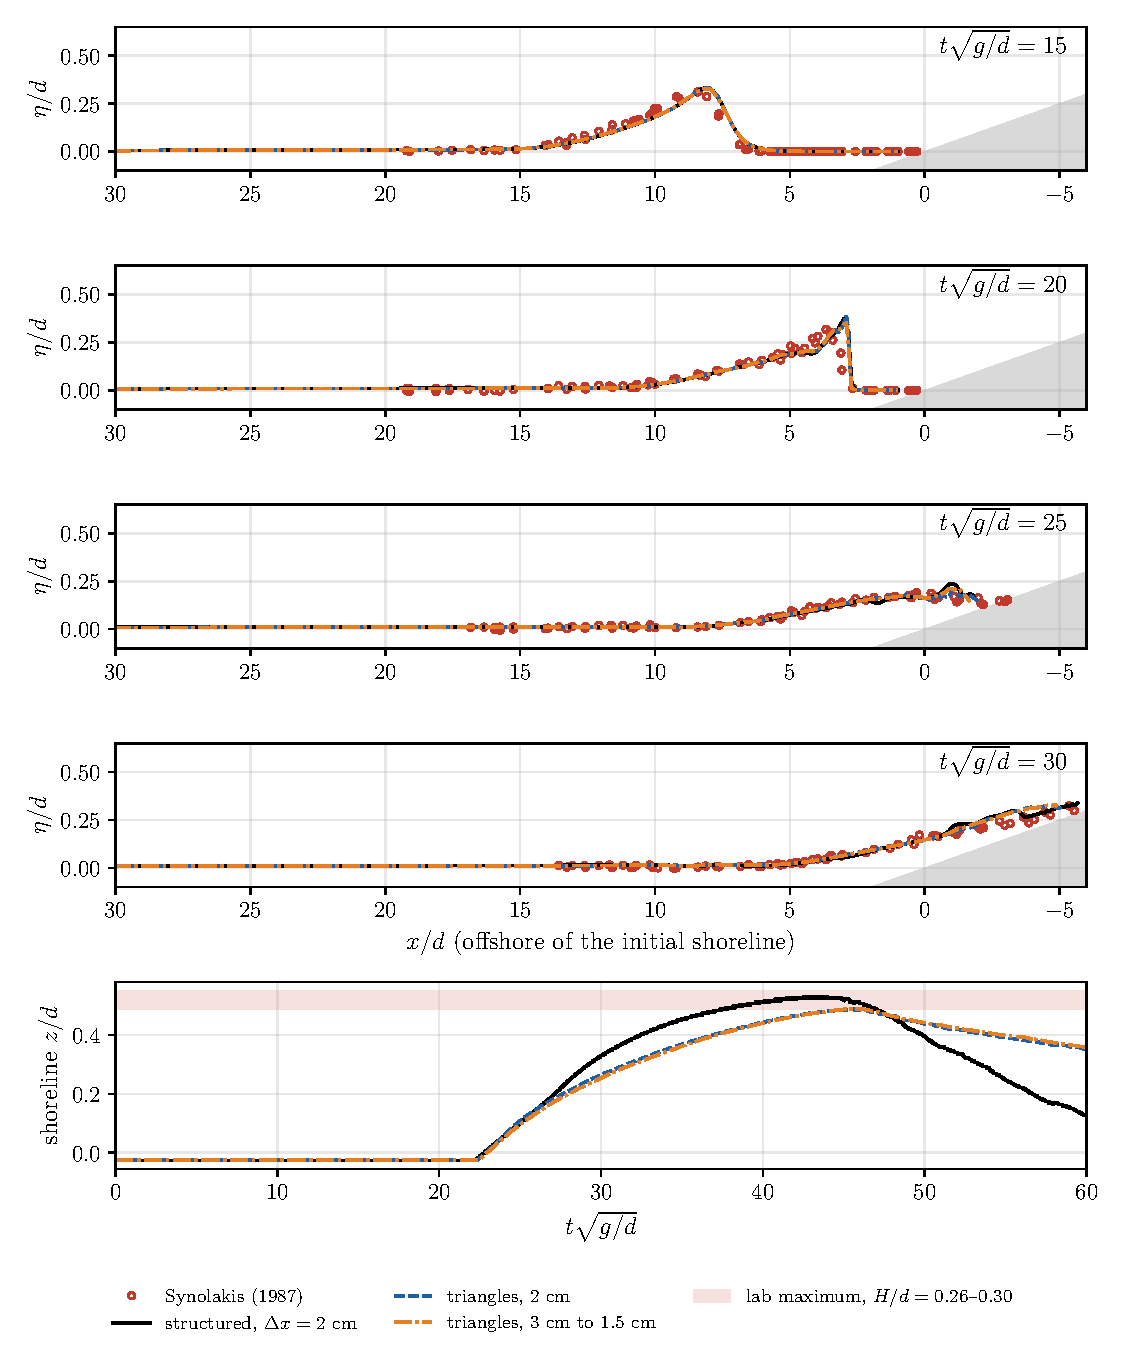
\includegraphics[width=0.85\textwidth]{unstructured_runup.pdf}
\caption{Solitary wave run-up ($H/d = 0.28$) on triangulated strips and on
the structured mesh: profiles averaged across the strip, and the shoreline
(highest wet bed) over time.}
\label{fig:unstr-runup}
\end{figure}

\paragraph{Diffraction by a vertical cylinder.} Regular waves of
$H = 1$ cm and $T = 1$ s in $h = 0.3$ m ($kh = 1.37$) from the boundary
wavemaker at $x = -3$ m meet a vertical cylinder of radius $a = 0.2$ m
($ka = 0.92$) at the origin. The half domain, 8 m by 4 m with a symmetry
wall on the axis and a 2.6 m sponge at the far end, has triangles of 2.5 cm
at the cylinder that grow to 6 cm 0.6 m away, and 4 layers (24\,289
triangles, 97\,156 prisms; Fig.~\ref{fig:cyl}a). The first-harmonic
amplitude over $t = 8$--12 s, after the waves have built up around the
cylinder and before those scattered back by the side wall and the
wavemaker return, is compared with the linear diffraction theory of
\citet{maccamy1954}. Around the cylinder the error is 0.07\,$a_I$ rms (at
most 0.095\,$a_I$); the run-up in front of it is 1.62\,$a_I$, against 1.71
(Fig.~\ref{fig:cyl}b). Along the axis in front of the cylinder the partial
standing wave has the right nodes and antinodes, the shadow behind it and
the pattern across are within a few percent of the theory, and over all 70
gauges the error is 0.06\,$a_I$ rms (Fig.~\ref{fig:cyl}c). In the window
that ends at 16 s the reflections from the walls of the half domain have
arrived (0.135\,$a_I$ rms around the cylinder). The run took 30 min on one
core for 16 s.

\begin{figure}[!htbp]
\centering
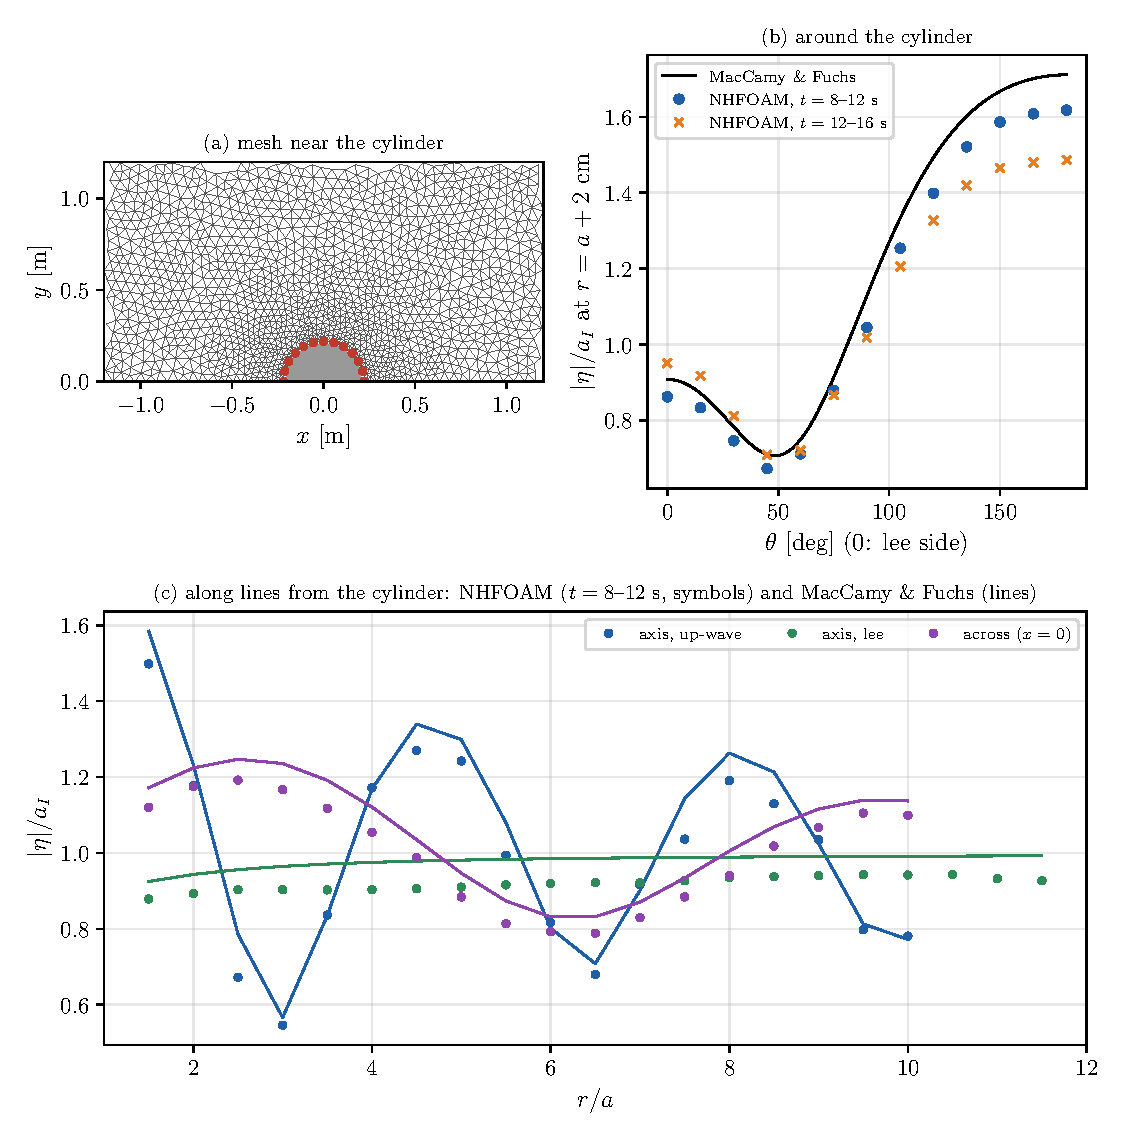
\includegraphics[width=0.78\textwidth]{cylinder_diffraction.pdf}
\caption{Diffraction by a vertical cylinder ($kh = 1.37$, $ka = 0.92$):
(a) the triangulated mesh near the cylinder and the gauges at
$r = a + 2$ cm; (b) amplitude around the cylinder; (c) amplitude along the
axis and across, against the theory of \citet{maccamy1954}.}
\label{fig:cyl}
\end{figure}

\subsection{Parallel runs, restarts and regression tests}
\label{sec:robust}
\label{sec:brk-par}

\paragraph{Breaking across processor boundaries.} A breaker that crosses a
processor boundary must be flagged as in a serial run: the flags spread
over neighbouring columns, and the persistence threshold depends on the age
of the breaking event, which travels with the wave. Ting \& Kirby's beach
with the default breaking model, run for 20 s on two processors with the
boundary at $x = 8$ m in the surf zone, now reproduces the serial run to
$4\times10^{-7}$ m at all gauges; before the ages were exchanged through the
processor patches (Section~\ref{sec:numhfa}) the difference reached 3.0 cm.
Gauges on a face between two columns are now always given to the same
column (the first one, also across processors), so that the records do not
depend on the rounding of the mesh points.

\paragraph{Restarts.} \NHFOAM\ writes its state with the fields: the time
levels of $\eta$, the face velocities of the last two levels, the surface
pressure unknowns, the breaking flags and ages, and the averaging time
(\code{uniform/NHFOAMState}). A restarted run keeps the mesh it was written
with and continues the BDF2 integration and the flux extrapolation. Ting \&
Kirby's beach (breaking, wetting and drying, averaging) restarted after 6 s
matches the continuous run to $6\times10^{-14}$ m in $\eta$ after another
6 s, and the bottom uplift to $10^{-18}$ m; without the state (Euler first
step, mesh placed on $\eta$) the differences were 2.5 mm and 4 cm/s. This
needs the fields at full precision (17 digits or binary): with 10 digits the
written state differs by $10^{-10}$, and the on/off breaking flags amplify
that to millimetres within seconds.

\paragraph{Regression suite.} \code{validation/regression.py} runs twelve short
cases in about three minutes on one core (standing and solitary waves, the
boundary wavemaker with regular and irregular waves and with measured
elevation and paddle records, a dam break and the
run-up with wetting and drying, breaking on Ting \& Kirby's beach, the
$k$--$\omega$ model, a bottom uplift and the triangulated beach) and compares
the extremes and final values of their gauge records with stored references.
It also checks that the breaking case run on two processors (with the
\code{structured} decomposition, the boundary near the breaking point) and
restarted at half time reproduces the serial, continuous run: to
$2\times10^{-7}$ m and $10^{-12}$ m.

\paragraph{Parallel speed-up.} On an otherwise idle machine with two cores
and the \code{structured} decomposition, Ting \& Kirby's beach with
breaking and wetting and drying (9200 cells, 10 s) took 102 s on one core
and 62 s on two (speed-up 1.64), and the 3D landslide tutorial (35\,280
cells, 4 s) 252 s and 131 s (1.92); the parallel runs reproduce the serial
ones to $3\times10^{-8}$ and $9\times10^{-8}$ m. The smaller 2DV case loses
more to the exchanges of the interface matrix and the breaking flags per
step.
